 \section{Systemidentifikation}
    \subsection{Modelle}
        In der Regelungstechnik arbeitet man mit verschiedenen Modellen. Generell unterscheidet man zwischen folgenden drei Arten.
        \subsubsection{White Box model} 
         \begin{wrapfigure}[5]{r}{0.4\linewidth}
                \vspace{-6mm}
                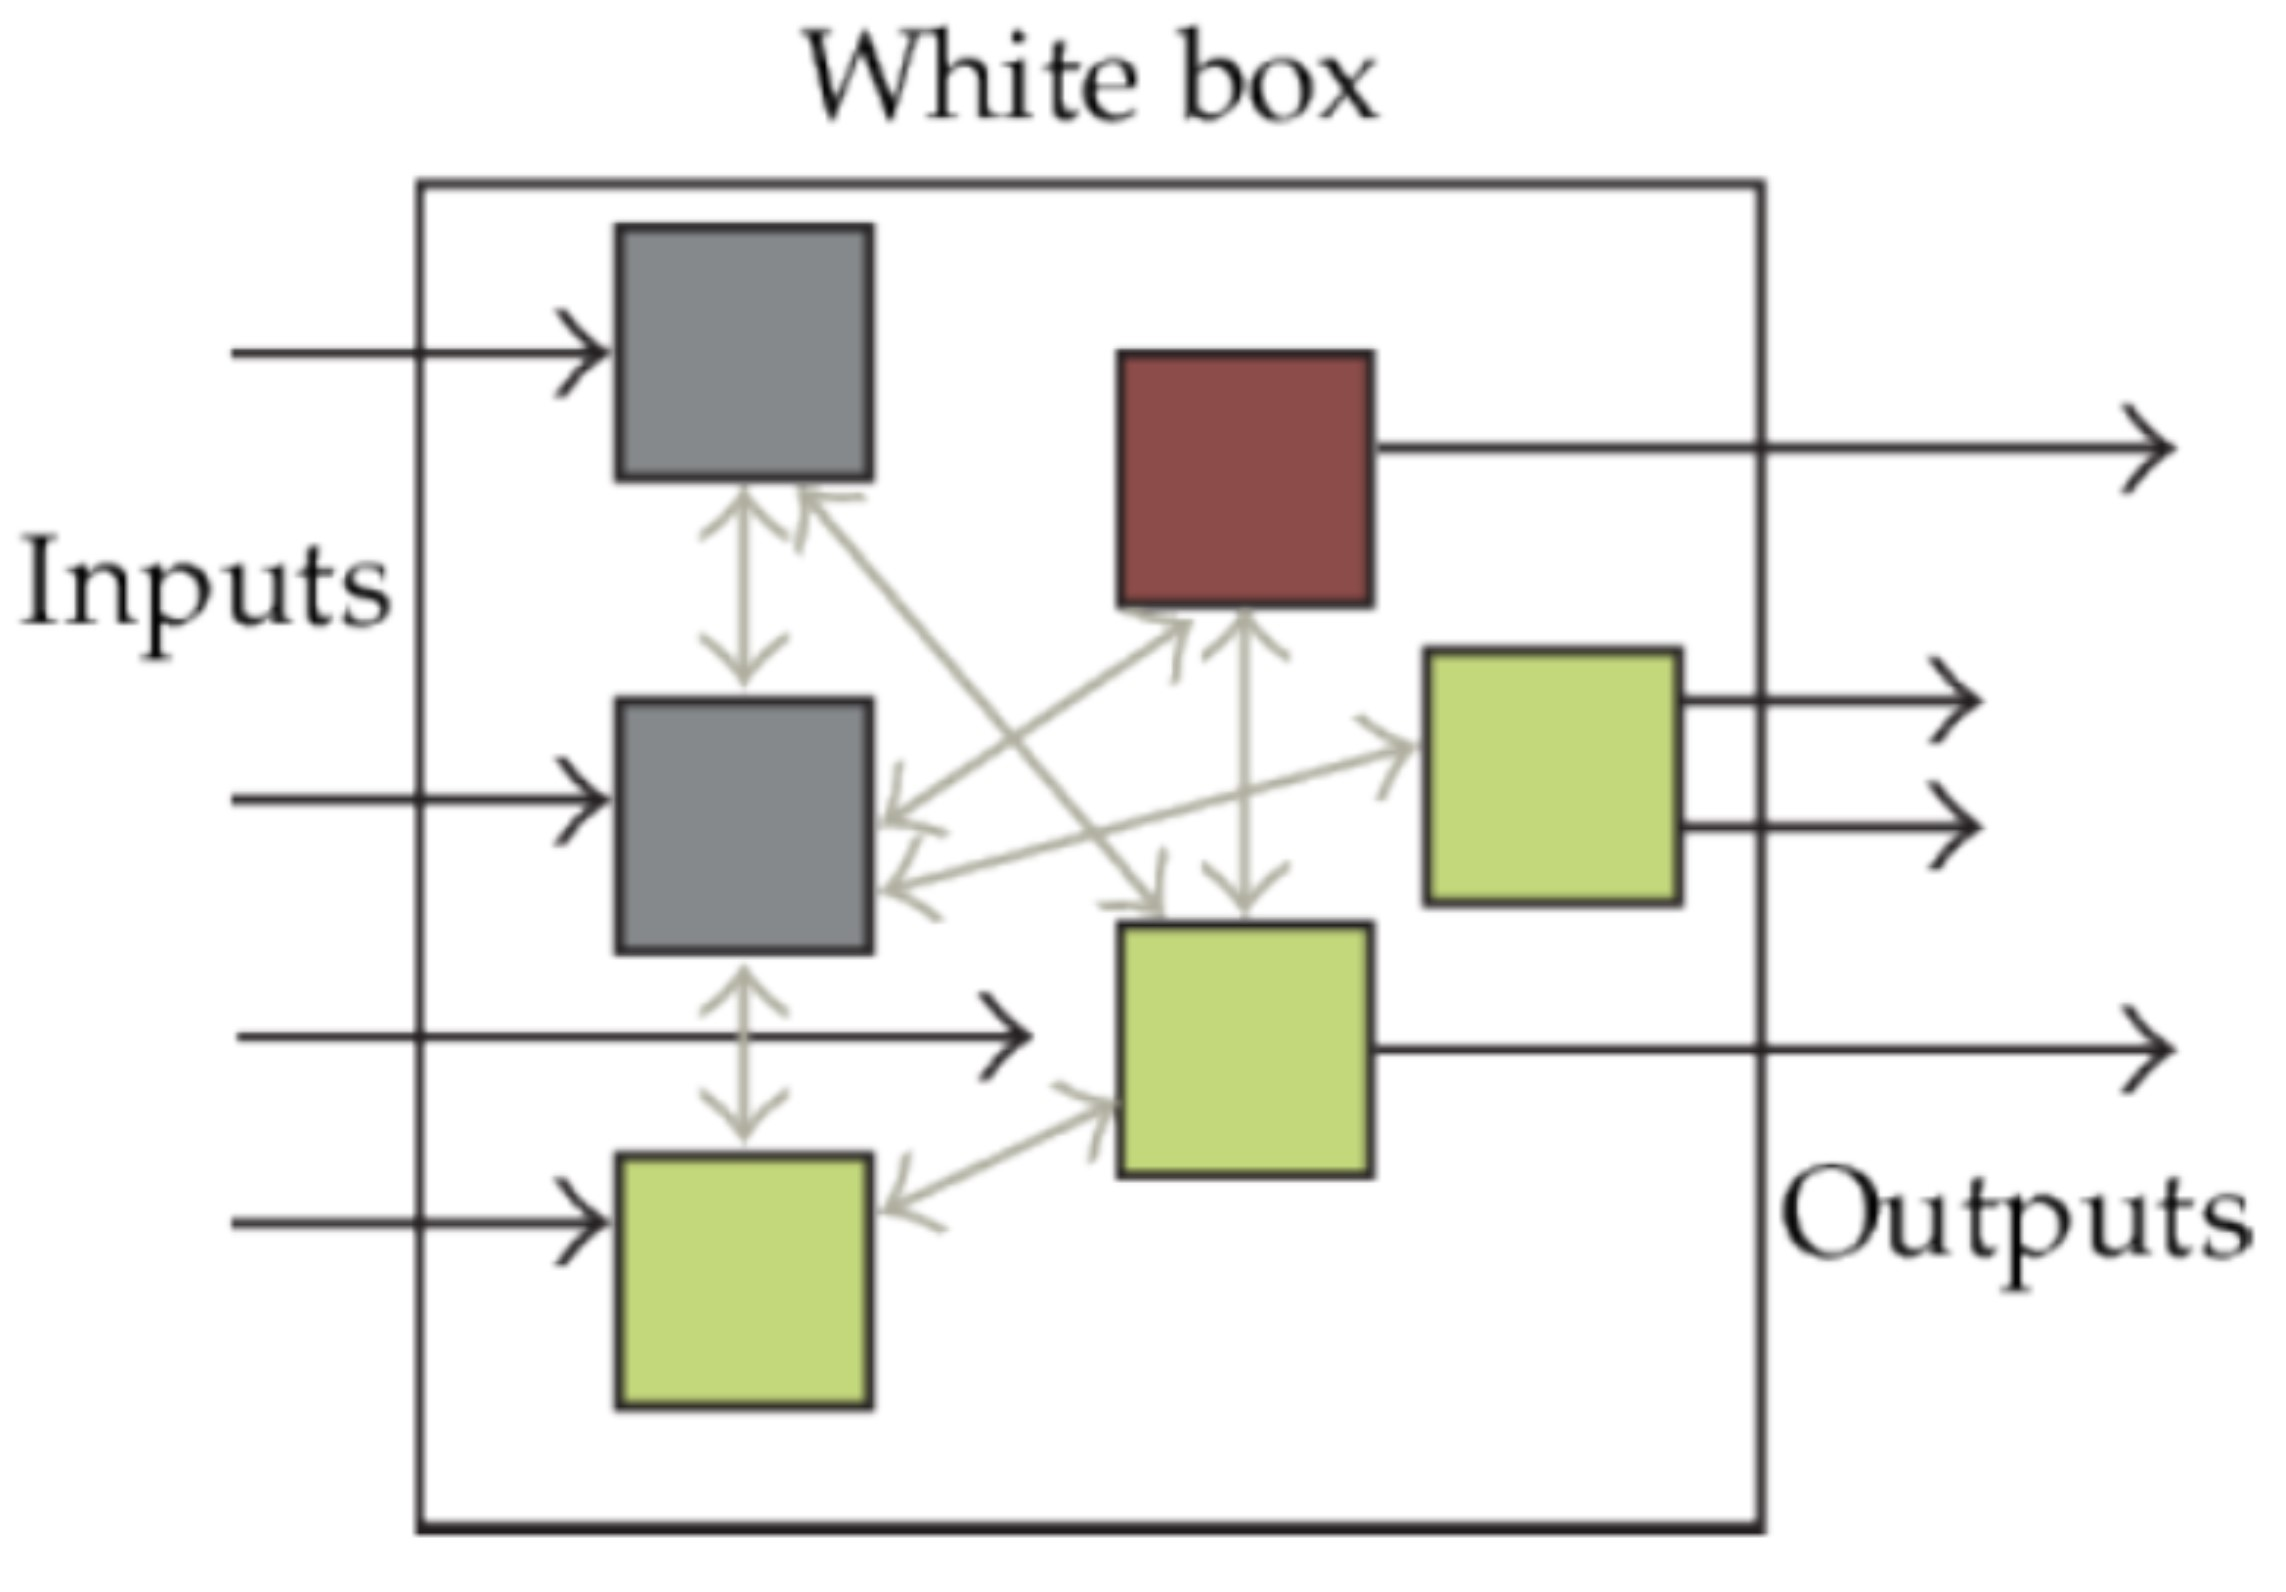
\includegraphics[width=\linewidth]{images/06/Whitebox.jpg}
            \end{wrapfigure}
            Es existiert eine Explizite Darstellung der Physik des Systems mit bekannten Parameterwerten.Das Verhalten, die Werte und der Zusammenhang zwischen den Zuständen ist vollständig bekannt.
        \subsubsection{Grey Box model}
            \begin{wrapfigure}[5]{r}{0.35\linewidth}
                \vspace{-6mm}
                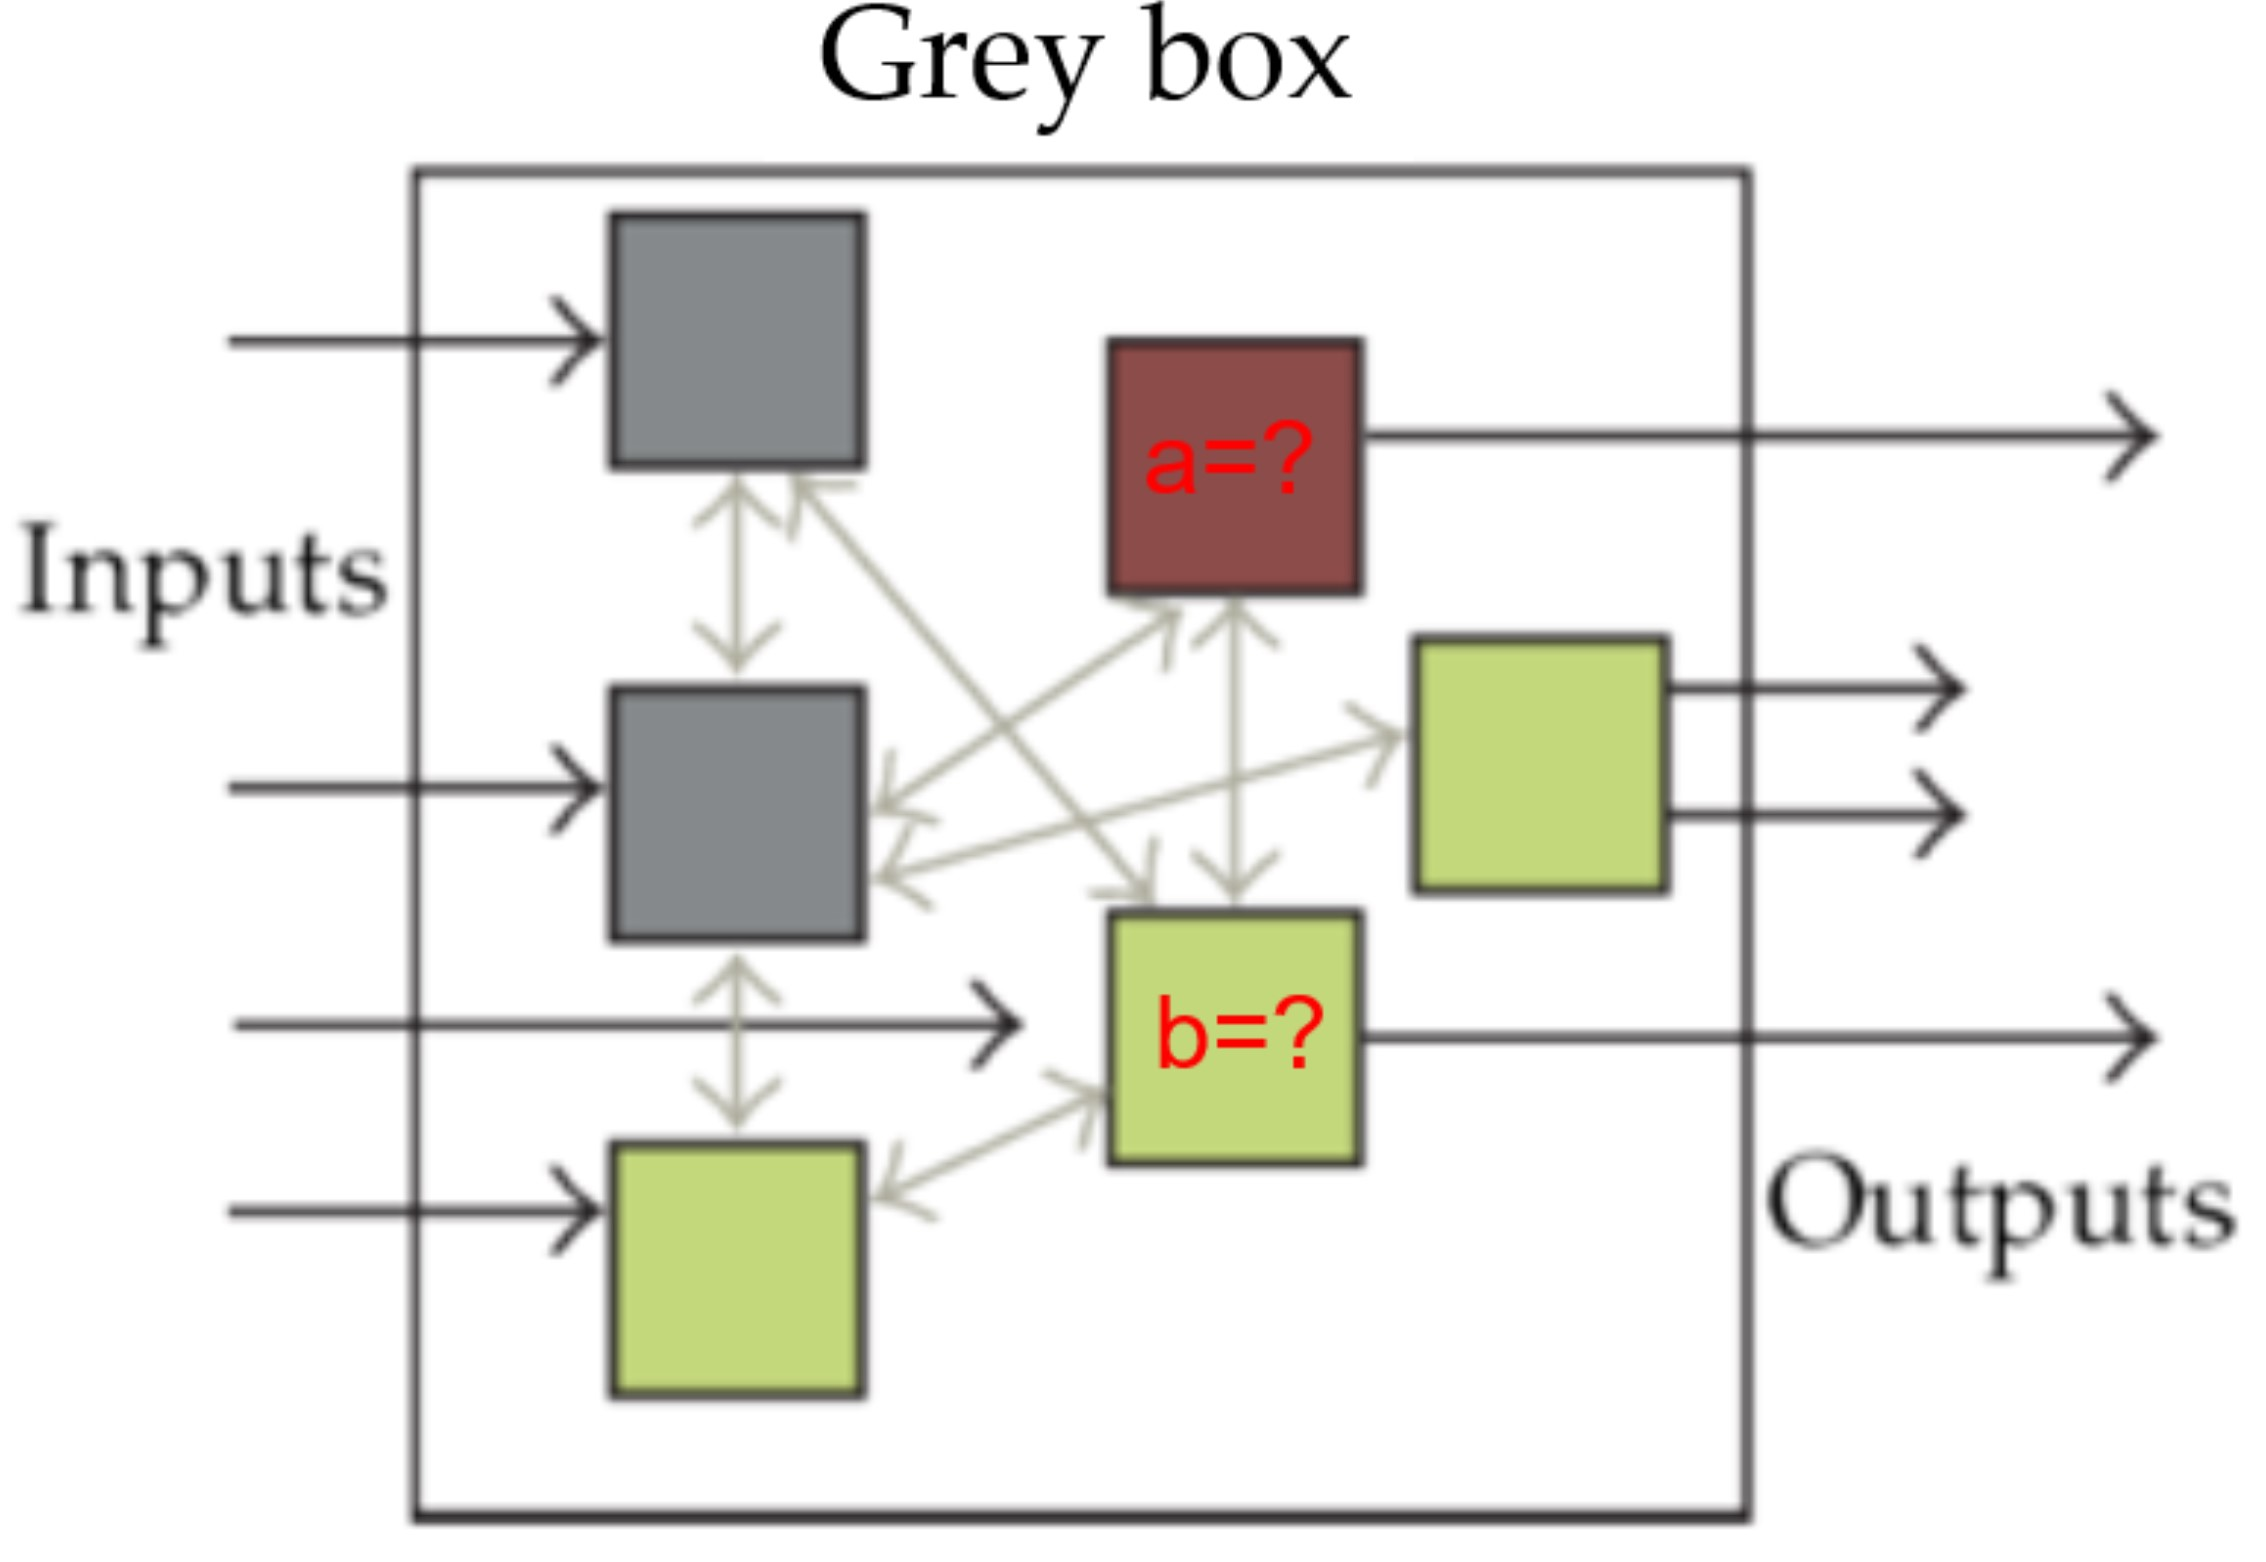
\includegraphics[width=\linewidth]{images/06/Greybox.jpg}
            \end{wrapfigure}
            Es existiert eine explizite Darstellung der Physik des Systems mit \textit{unbekannten} Parameterwerten. Die Zusammenhänge und Verhalten der Zustände sind jedoch bekannt.\\
            
            
           
        \subsubsection{Black Box model}
            \begin{wrapfigure}[4]{r}{0.3\linewidth}
                \vspace{-6mm}
                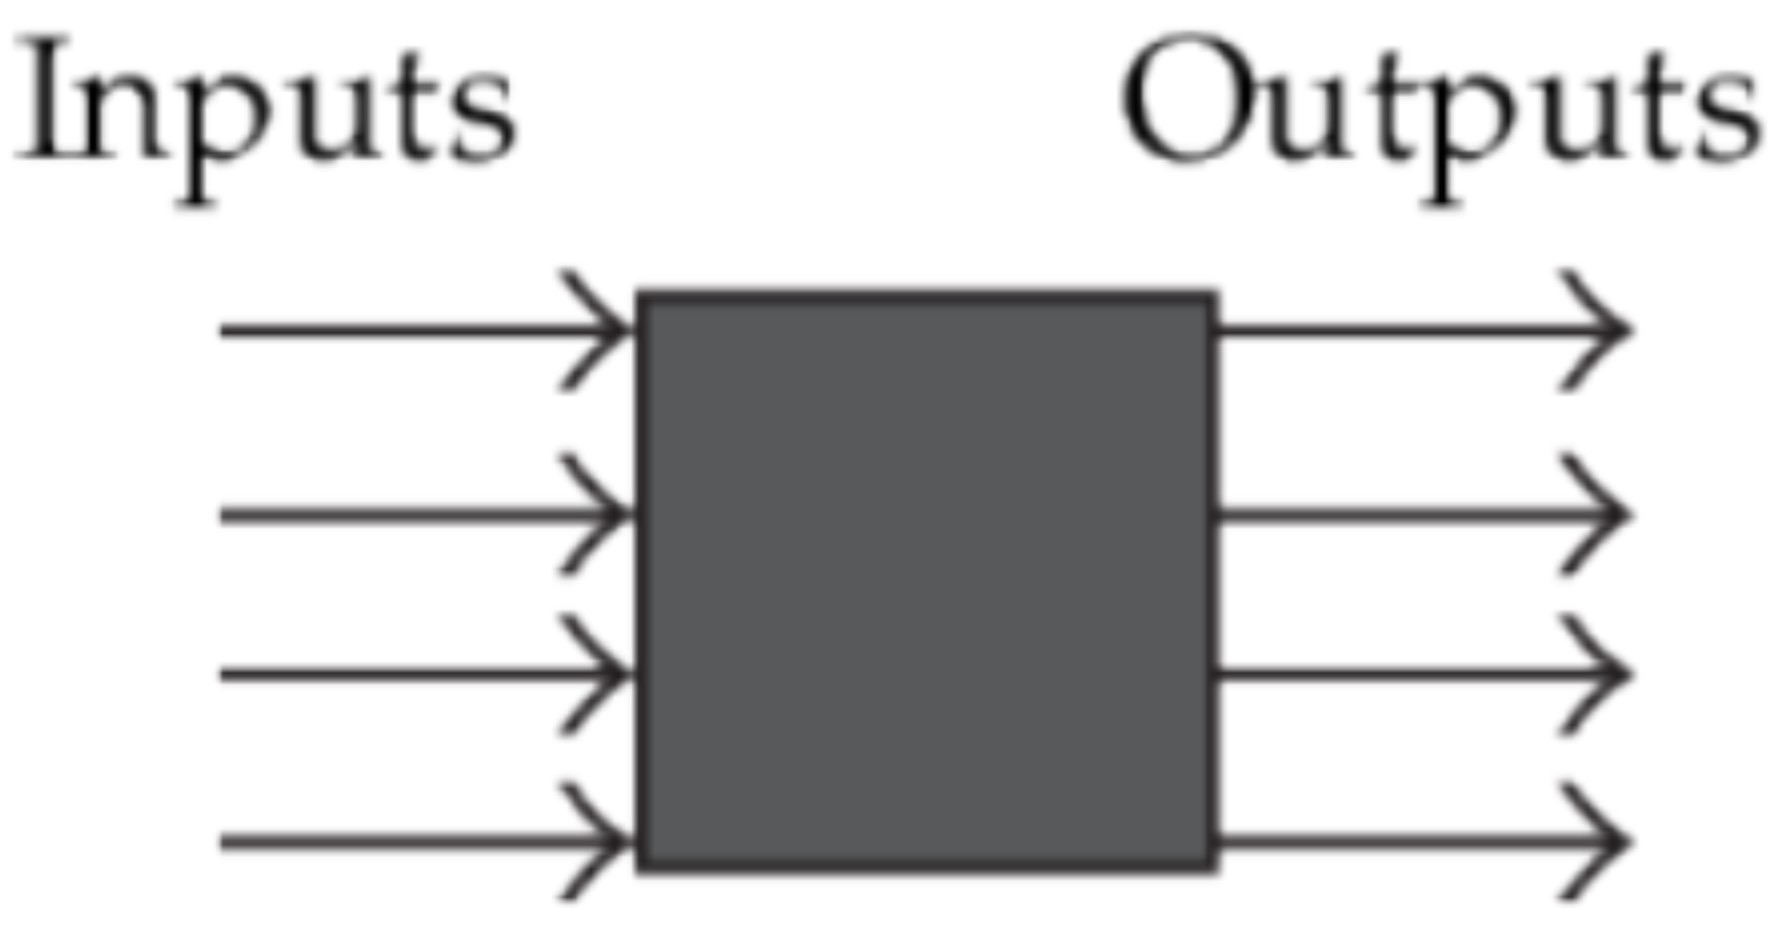
\includegraphics[width=\linewidth]{images/06/Blackbox.jpg}
            \end{wrapfigure}
            Es existiert keine explizite Darstellung der Physik des Systems. Das Systemverhalten muss durch empirische Datenanalyse ermittelt werden. 
           
            Black box Modelle werden verwendet wenn die Physik des Systems nicht genau bekannt oder zu komplex ist um einfach modelliert zu werden. Durch experimentelle Modellbildung (Systemidentifikation) kann ein Modell des Systems abgeleitet werden, das für die Reglerentwicklung erforderlich ist. 
            
        \subsubsection{Systemidentifikation mittels Frequenzgang}
            Ein unbekanntes System kann wie folgt identifiziert werden:
            \begin{enumerate}
                \item Das System wird mit einem bekannten harmonischen Eingangssignal angeregt: $u(t) = cos(\omega t),\omega \in [0,\infty).$
                \item Die Verstärkung $|\Sigma(j\omega)|$ und die Phase $\angle\Sigma(j\omega)$ der Systemantwort $y_\infty = |\Sigma(j\omega)| \cdot cos(\omega t + \angle\Sigma(j\omega))$ werden gemessen. Somit kann das Bodediagramm des Systems experimentell bestimmt werden.
                \item Eine Übertragungsfunktion wird an die Daten angepasst. Hier ist es wichtig, die Auswirkung verschiedener Standardelementen auf Magnitude und Phase zu verstehen.
            \end{enumerate}